% !TEX root = ../entropy.tex

\section{Data}%
\label{sec:data}

\subsection{Preprocessing}%
\label{sub:preprocessing}

Duplicate transactions


\subsection{Sample selection}%
\label{sub:sample_selection}

\begin{table}[ht]
\caption{Sample selection}\label{tab:selection}
\begin{tabular}{lrrrr}
\toprule
                                                 &  Users & Accounts & Transactions & Value (\pounds M) \\
\midrule
                                      Raw sample & 24,163 &  123,625 &   59,647,019 &          11,209.7 \\
                       At least 6 months of data & 21,508 &  117,000 &   59,088,076 &          11,116.8 \\
                               No missing months & 18,550 &   98,513 &   51,252,412 &           9,606.4 \\
                      Account balances available & 14,714 &   85,590 &   44,163,629 &           8,618.7 \\
At least 5 debits totalling \pounds200 per month & 12,296 &   70,981 &   38,618,825 &           7,469.7 \\
                    At least one current account & 12,148 &   70,366 &   38,280,116 &           7,421.9 \\
            Income in 2/3 of all observed months &  9,963 &   60,151 &   33,270,455 &           6,490.2 \\
 Yearly income between \pounds5k and \pounds200k &  6,716 &   36,829 &   21,460,727 &           3,677.9 \\
            No more than 10 accounts in any year &  6,169 &   26,999 &   18,241,355 &           2,855.1 \\
      Debits of less than \pounds100k each month &  5,760 &   24,486 &   16,409,561 &           1,998.7 \\
                                    Final sample &  5,760 &   24,486 &   16,409,561 &           1,998.7 \\
\bottomrule
\end{tabular}

\end{table}


\subsection{Dataset description}
\label{sub:dataset_description}

Data is provided by Money Dashboard (MDB), a UK-based
financial management app that allows its users to add accounts from all
their banks to obtain an integrated view of their finances. Our
dataset contains information on more than 500 million transactions made between
2012 and June 2020 by more than 250,000 users. For each transaction, we can see
the amount, date, and description of the transaction, as well as transaction
\textit{tags}, classifications added by MDB that indicate the type of the
transaction (e.g.  `groceries', `insurance'). We also have basic information
 on each user (e.g. year of birth, postcode sector) as well information about
each bank account (e.g. type of account, date added).

\begin{figure}
    \caption{Demographic characteristics of Money Dashboard users}
    \label{fig:sumstats}
    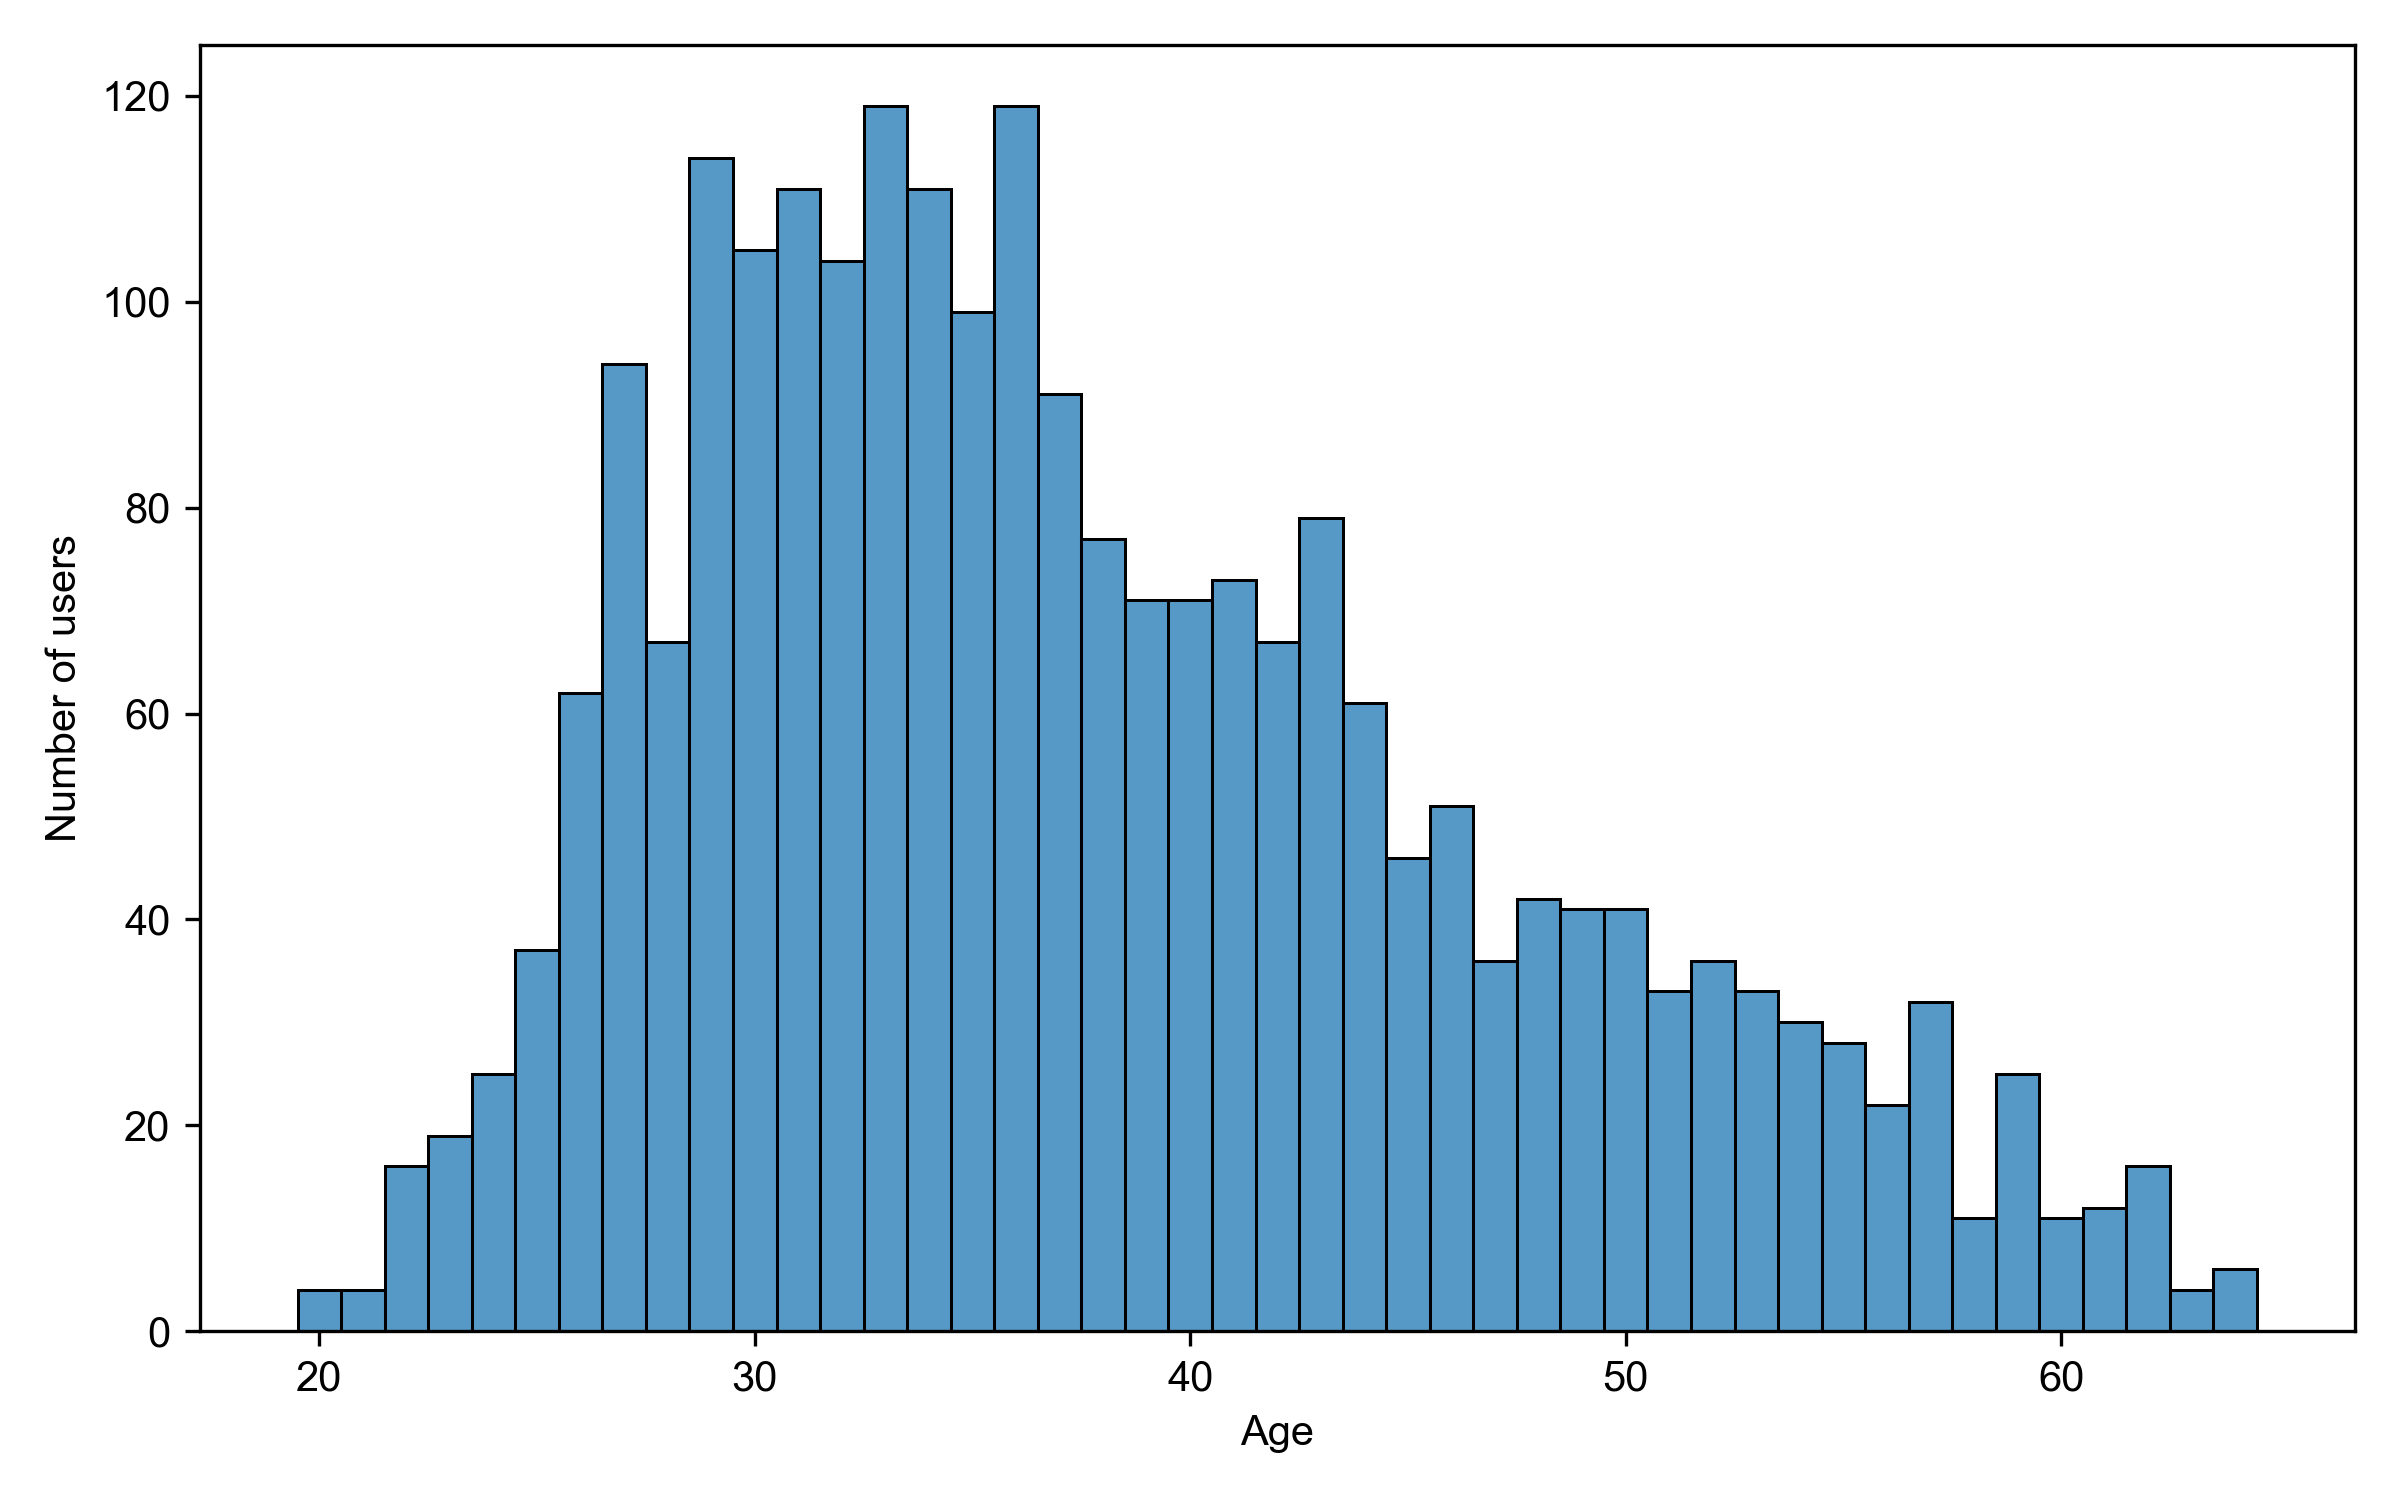
\includegraphics[width=0.49\textwidth]{\figdir/user_age_hist.png}
    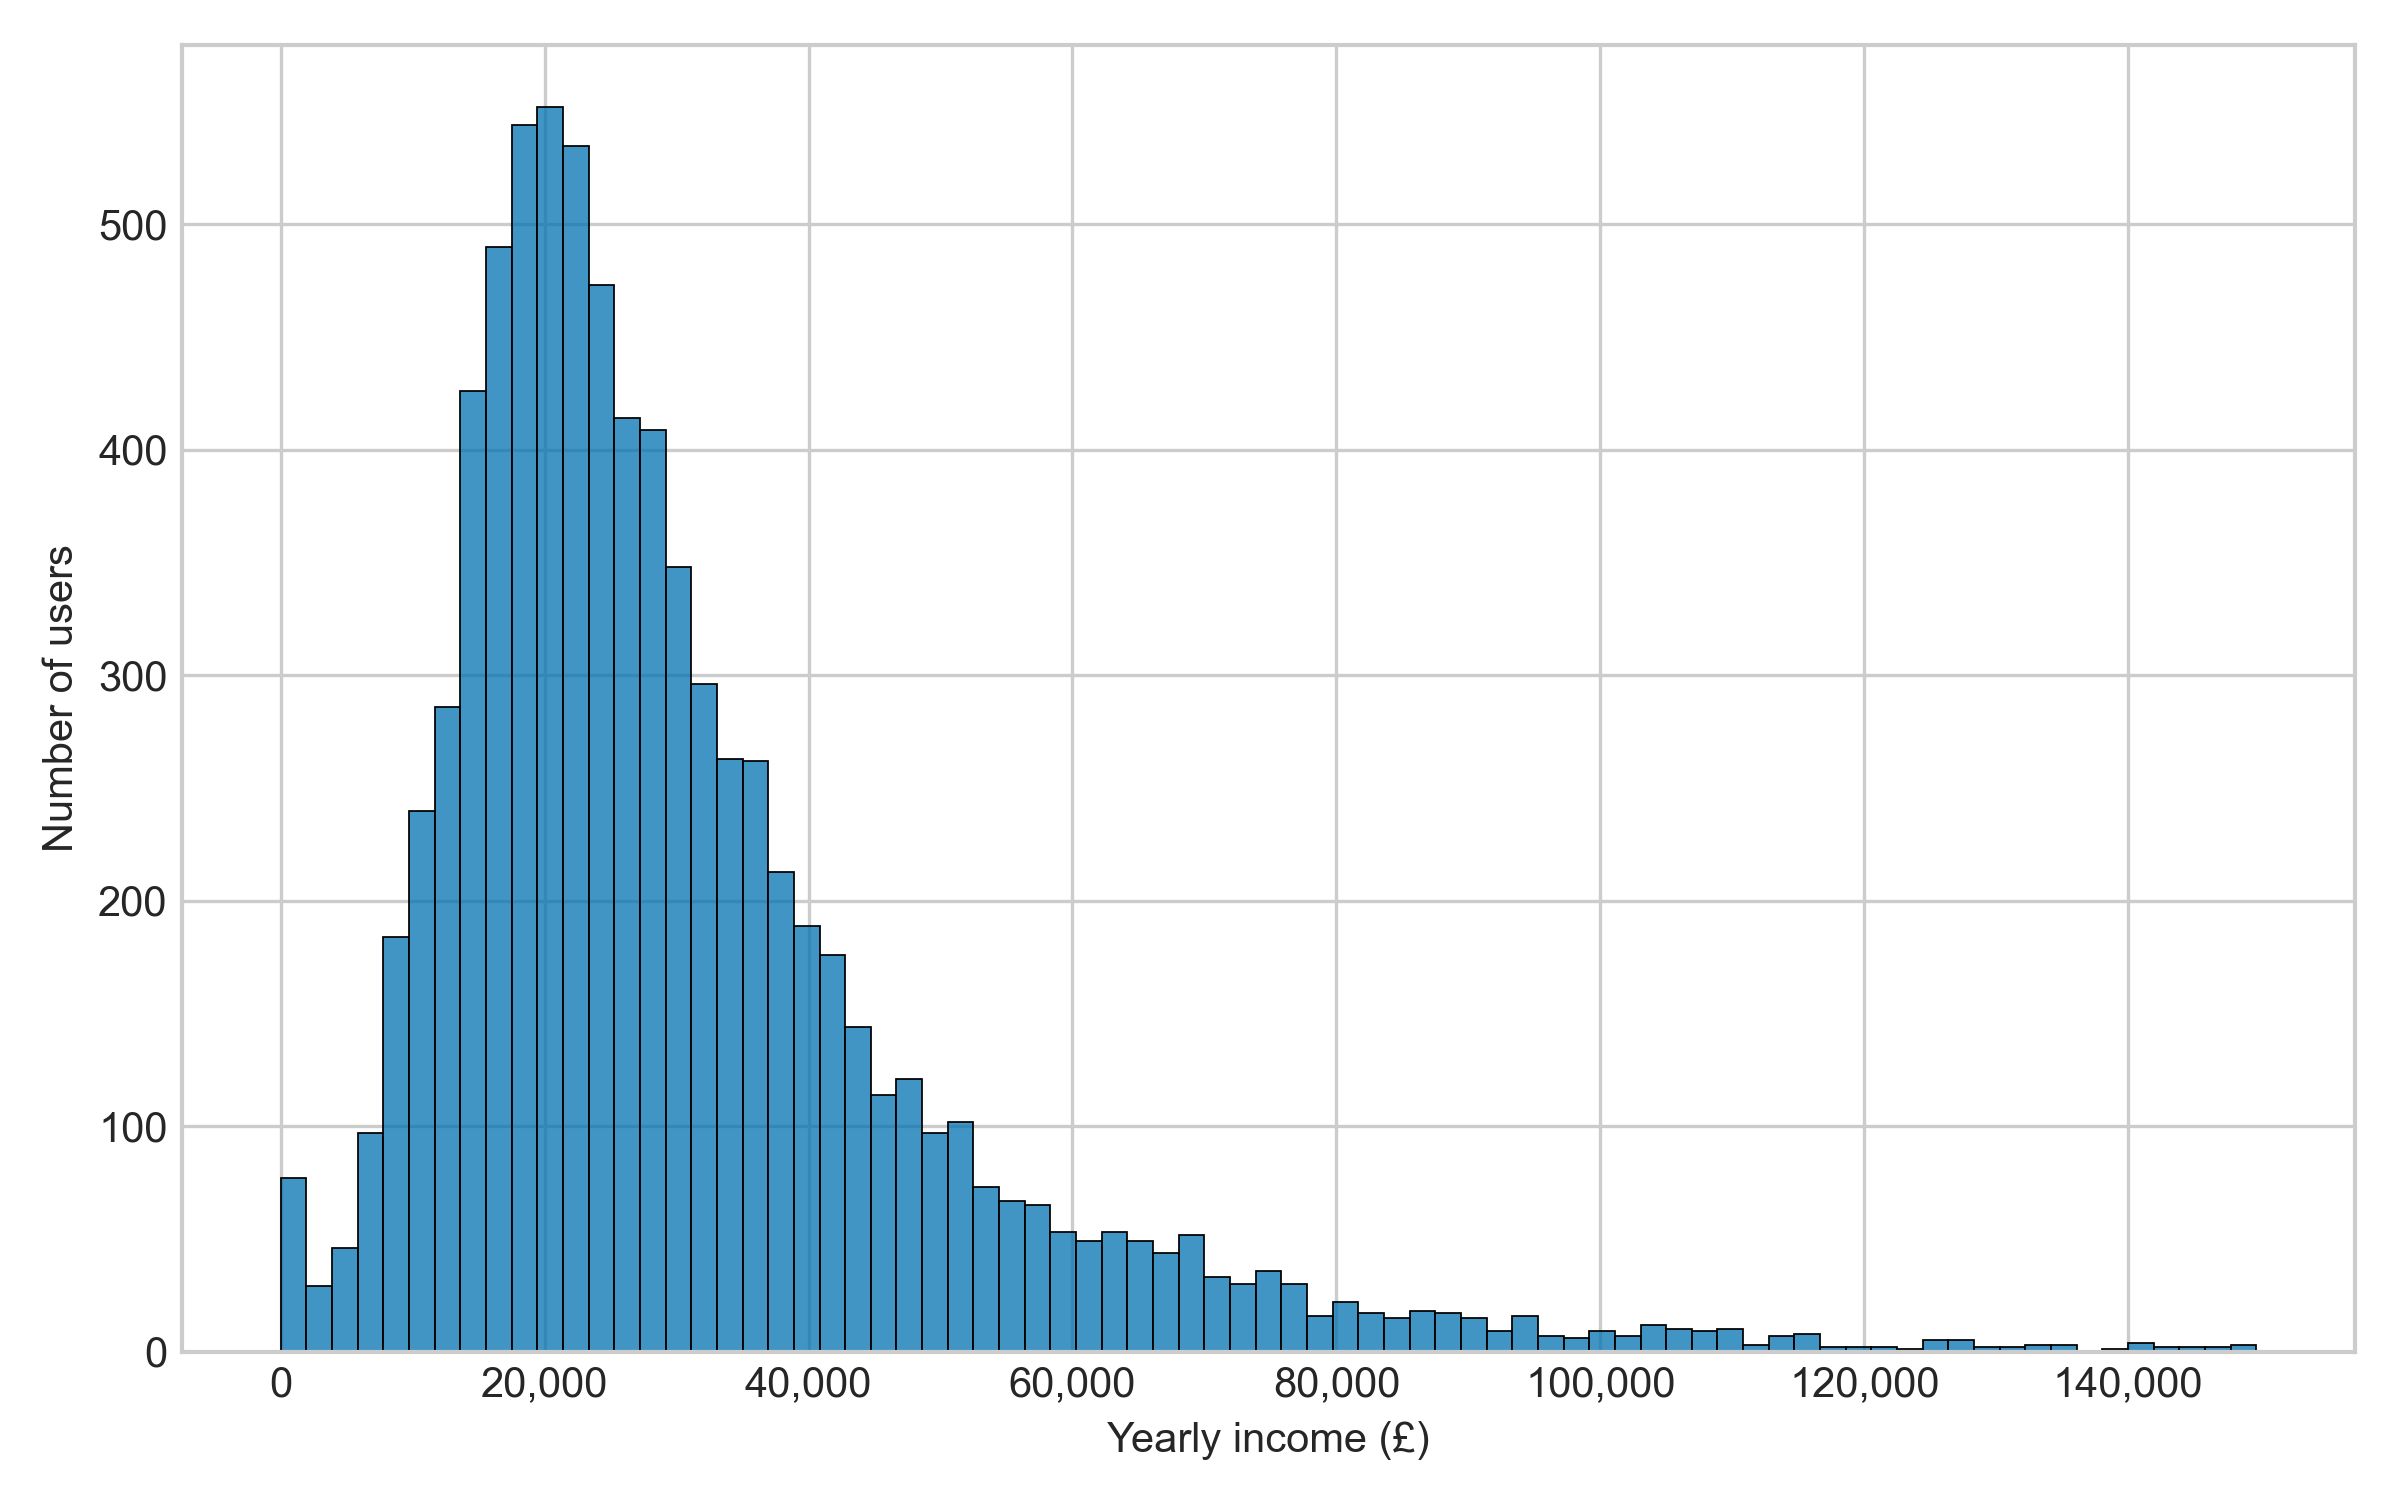
\includegraphics[width=0.49\textwidth]{\figdir/user_income_hist.png}
    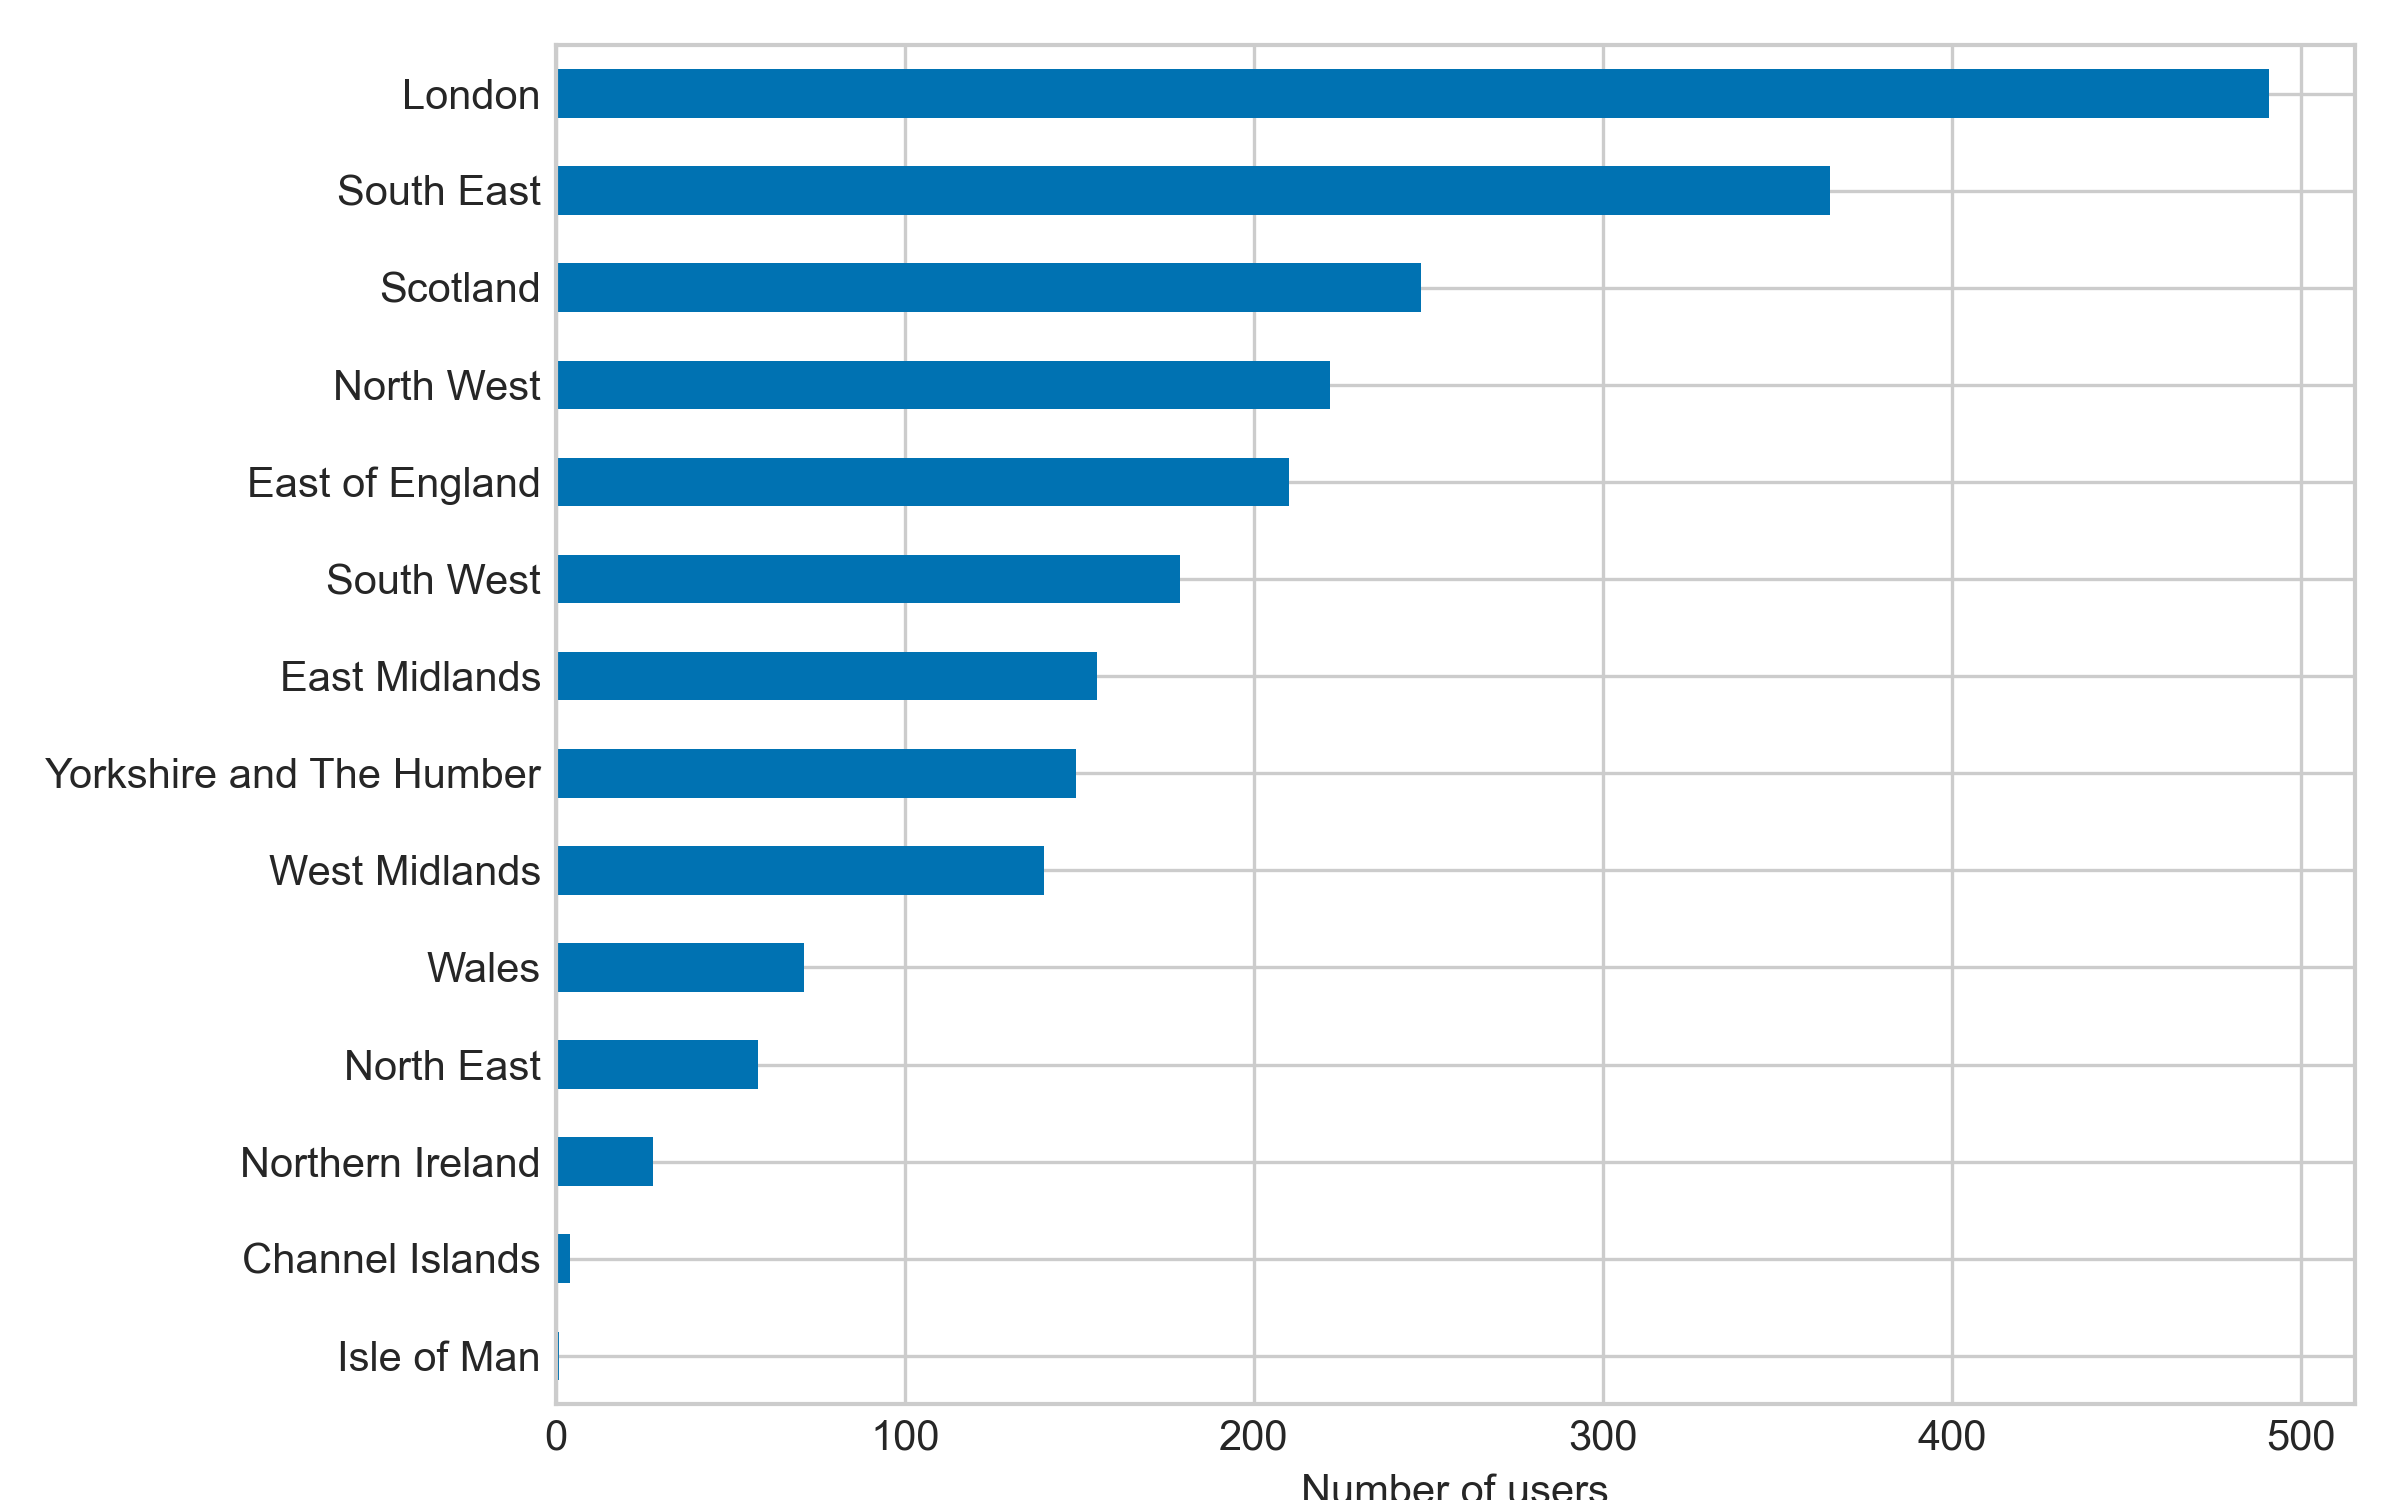
\includegraphics[width=0.49\textwidth]{\figdir/user_region_distr.png}
    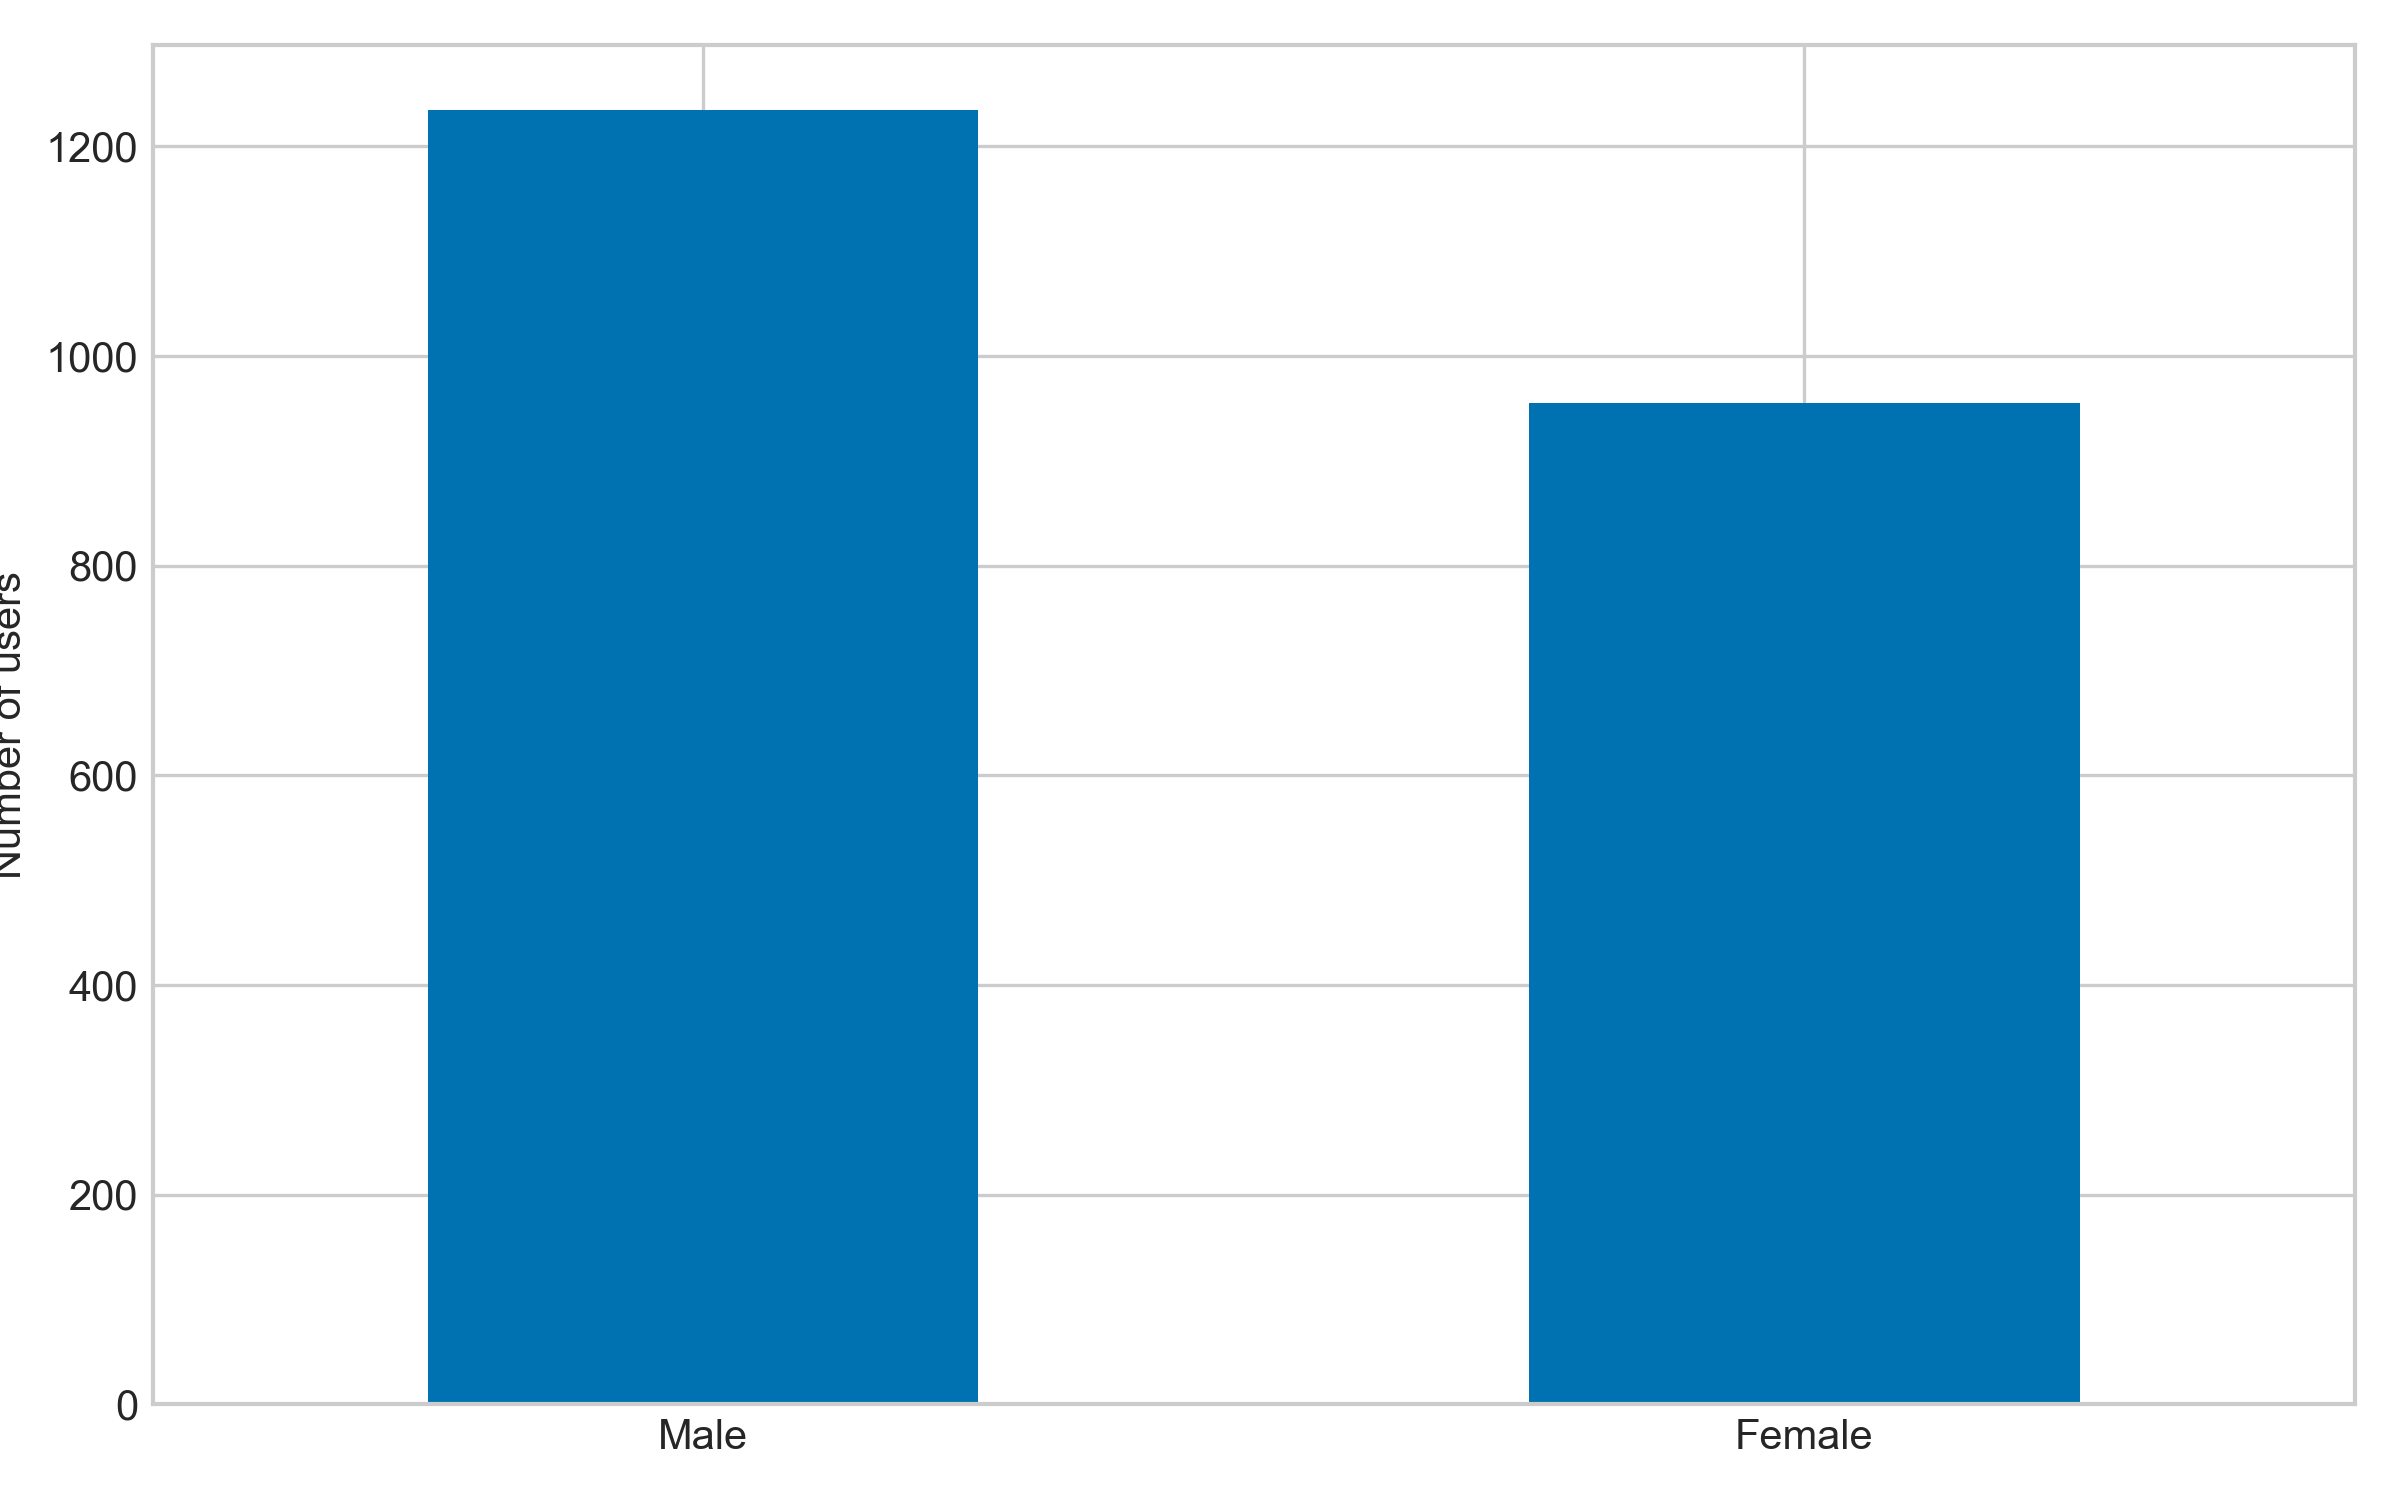
\includegraphics[width=0.49\textwidth]{\figdir/user_gender_distr.png}
\end{figure}

The main advantages of the data for the study of consumer financial behaviour
are its high (transaction-level) frequency, that it is automatically
collected and updated and thus less prone to errors and unaffected by biases
that bedevil survey measures, and that it offers a view of consumers' entire
financial life across all their accounts, rather than just a view of their
accounts held at a single bank (provided they added all their accounts to MDB).

The main limitation is the non-representativeness of the sample relative to the
population as a whole. Financial management apps are known to be used
disproportionally by men, younger people, and people of higher socioeconomic
status \citep{carlin2019generational,mas2014money}, a fact that is reflected in
our data. The four panels in Figure~\ref{fig:sumstats} provide an overview of
demographic characteristics of our sample. It makes clear that Money Dashboard
users are not a representative sample of the UK population: they are
predominantly males in their thirties who live in London or the South East and
are relatively well off (the income distribution is shifted to the right
relative to the UK as a whole).\footnote{To calculate incomes, we broadly follow
    \citet{hacioglu2020distributional} in defining total income as the sum of
    earnings, pension income, benefits, and other income.
    % We define these four
    % categories using the following tags: income: \textit{Salary or Wages
    % (Main)}, \textit{Salary or Wages (Other)}, and \textit{Salary (secondary)}
    % Pension income: \textit{Pension - other}, \textit{Pension}, \textit{Work
    % pension}, \textit{State pension}, \textit{Pension or Investments}: Benefits:
    % \textit{Benefits}, \textit{Family benefits}, \textit{Job seekers benefits},
    % \textit{Other benefits}, \textit{Incapacity benefits}: Other income:
    % \textit{Income}, \textit{Irregular Income or Gifts}, \textit{Miscellaneous
    % income - other}, \textit{Interest income}, \textit{Rental Income},
% \textit{Investment income - other}, \textit{Rental income (whole property)},
% \textit{Loan or Credit Income}, \textit{Bond income}, \textit{Dividend}.
} Also,
as pointed out in \citet{gelman2014harnessing}, a willingness to share financial
information with a third party might not only select on demographic
characteristics, but also for an increased need for financial management, or,
one could argue, for a higher degree of financial sophistication. However, while
non-representativeness could partially be addressed by re-weighting the sample,
as was done in \citet{bhourquin2020effects}, it is not of much consequence for
our purpose here, since our ability to infer behaviour traits from transaction
data is not dependent on having a representative sample of people.


\begin{figure}[h]\center \newcommand\width{.9\textwidth} \caption{Monthly
        transactions by account type}    \label{fig:monthly_txns}
        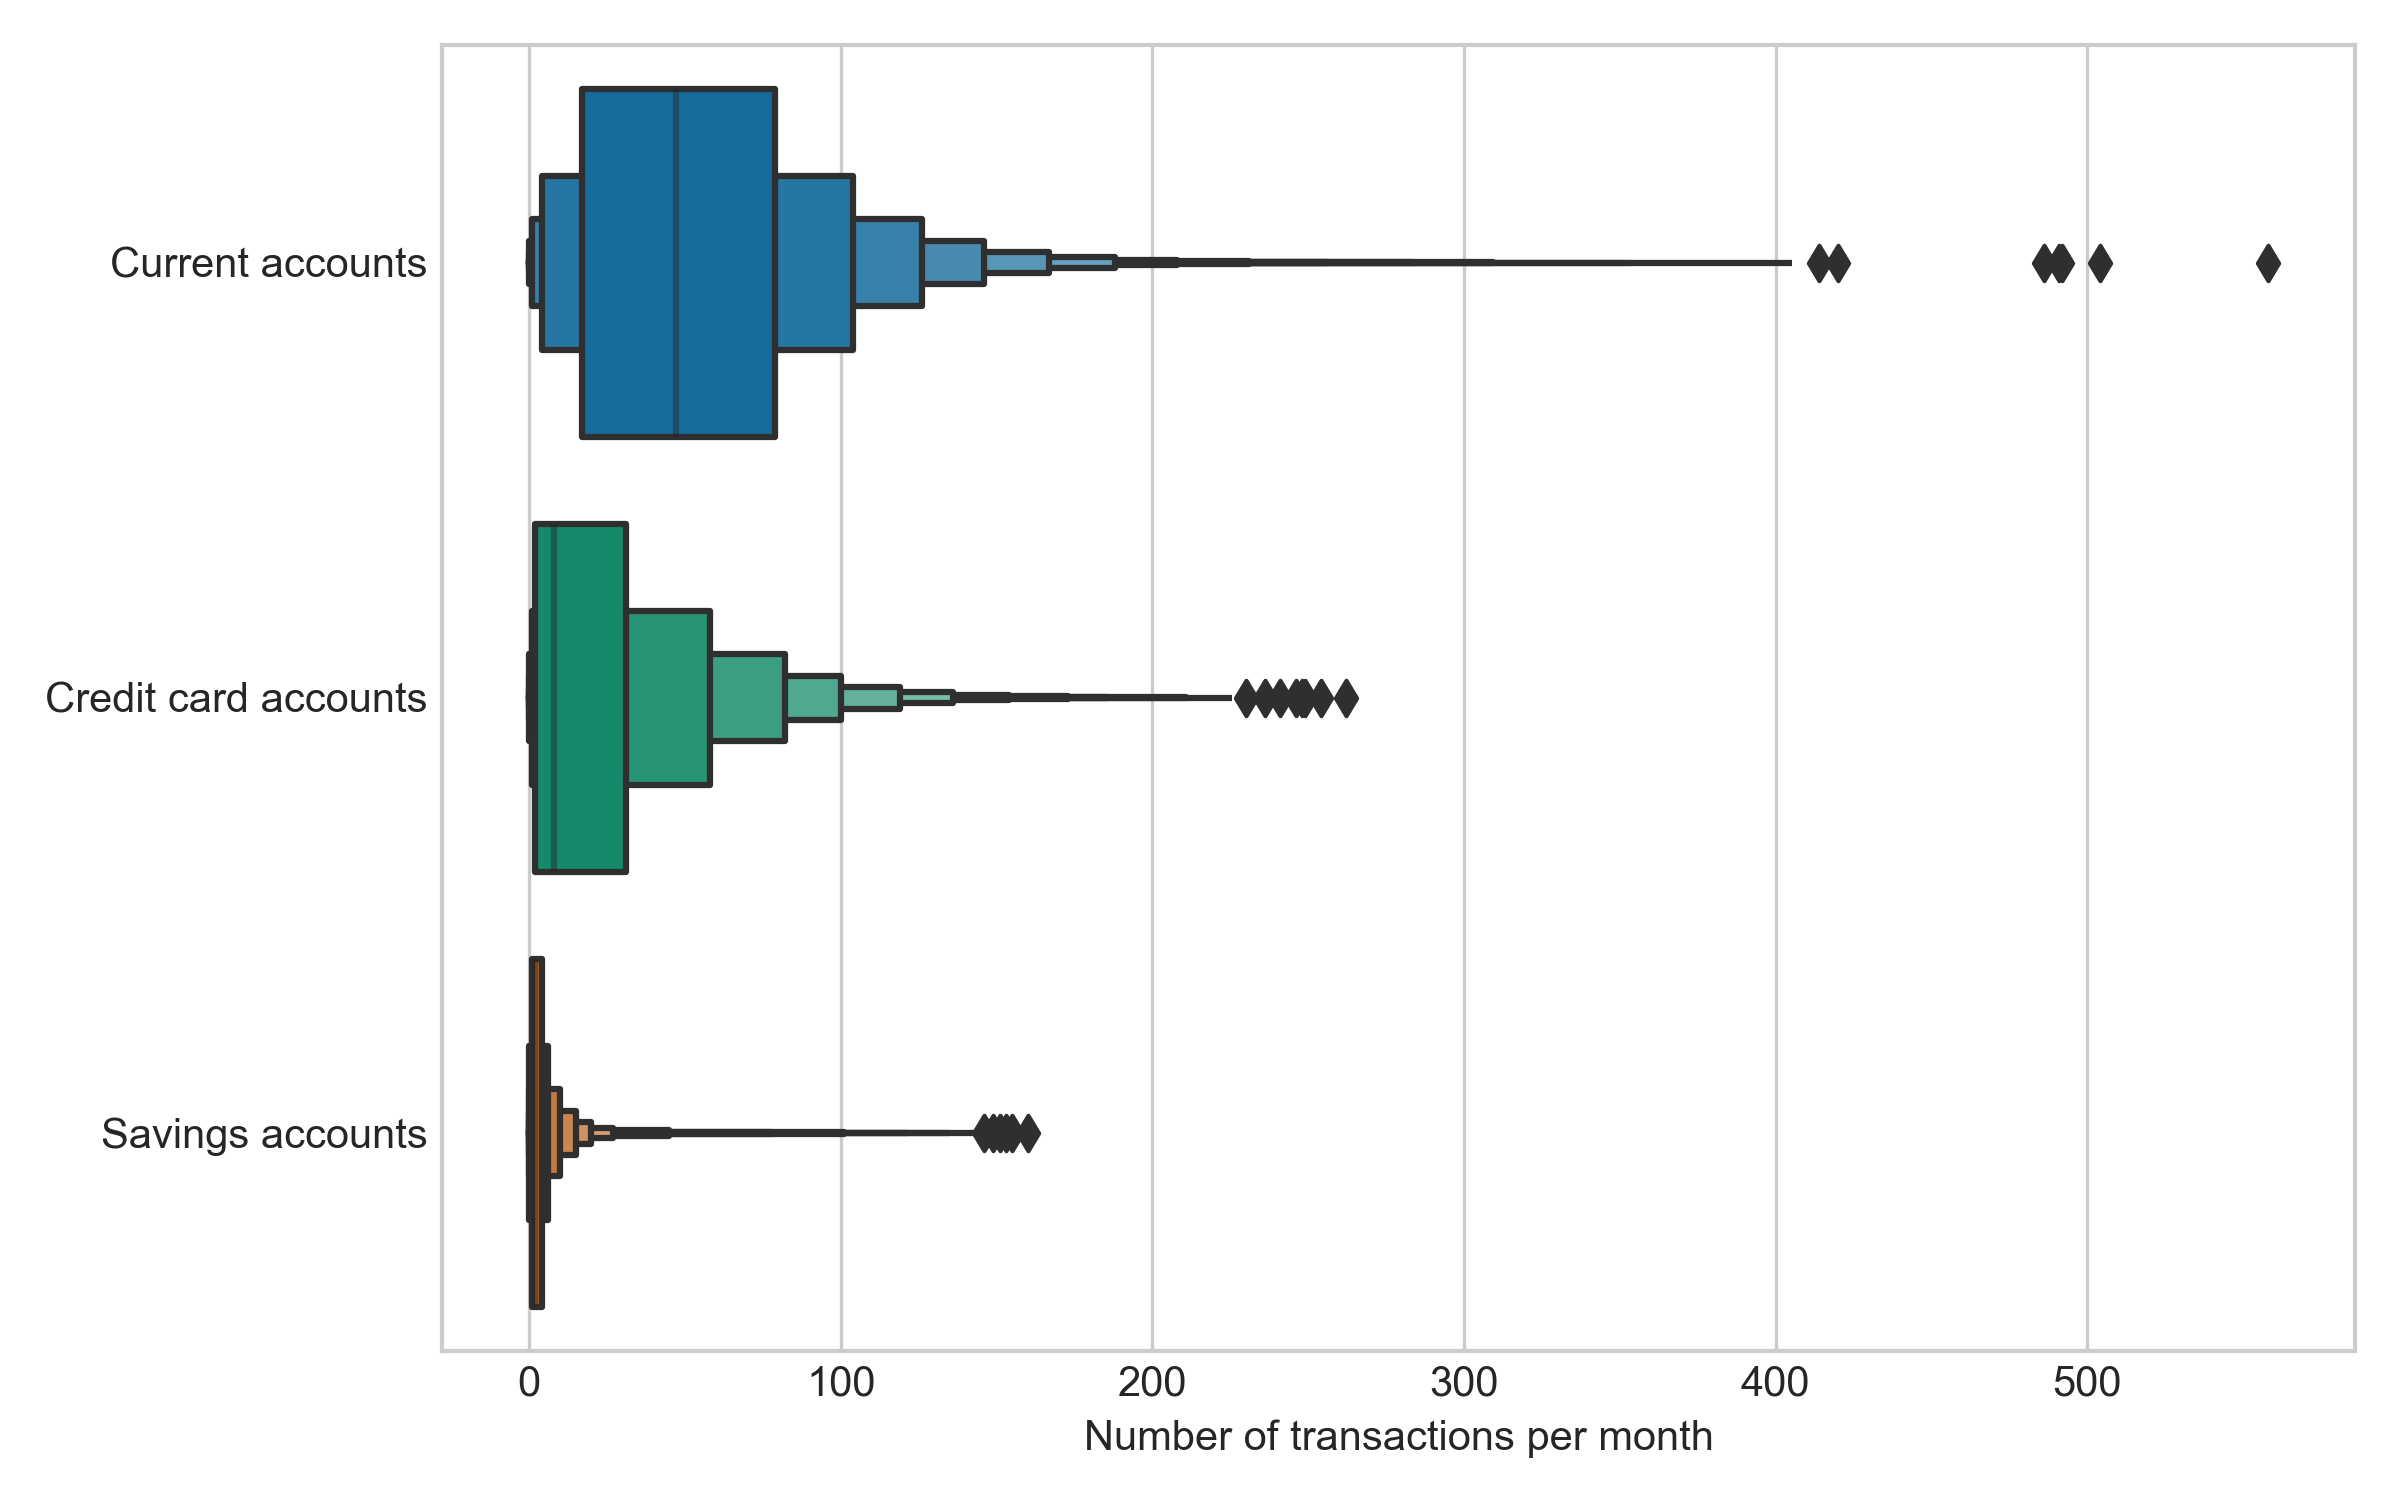
\includegraphics[width=\width]{\figdir/num_txns_by_account_type.png}
        \fignote{\width}{The two innermost boxes in the
            \href{https://vita.had.co.nz/papers/letter-value-plot.html}{letter-value
            plots} are identical to those in a boxplot, with the center line
            corresponding to the median and the left and right edges to the
            first and third quartiles, respectively -- or half of the remaining
            data on either side of the median.  Additional boxes on either side
            extend that principle by corresponding to half of the remaining
            data on that side. For instance, the second box to the right of the
            median in the current accounts plot indicates that half of all
            account-month observations to the right of the third quartile have
            fewer than about 105 transactions. Boxes of the same height
            correspond to the same level, individually drawn observations are
        outliers.}
\end{figure}



\subsection{Dependent variable}%
\label{sub:dependent_variable}

Types of balances, from \citet{becker2017does}, who treats balance at end of
each month as observations:

\begin{itemize}
    \item Current account balance
    \item Debit balance (savings and current account balance)
    \item Pure savings (savings account balance only)
    \item Credit balance (loans and negative current account)
    \item Pure credit (loans only)
    \item Wealth held (debit - credit balance)
\end{itemize}


\subsection{Independent variable}%
\label{sub:independent_variable}

Spending entropy:
\begin{itemize}
    \item We calculate spending entropy using the Shannon entropy
        \textit{H}\citep{shannon1948mathematical}, defined as
        \begin{equation}
            H = -\sum{p_i}log_2(p_i),
        \end{equation}
        where $p_i$ is the probability that an
        individual makes a purchase in spending category $i$. The measure can
        broadly be interpreted as the degree to which an individual's spending
        pattern is predictable, whith a higher score indicating less
        predictability.

    \item To calculate individual entropy scores, we group spending into 9
        spending categories (SC), based on the classification used
        by Lloyds Banking Group as discussed in \citet{muggleton2020evidence}.

    \item Also following that paper, when calculating $p_i$ we use additive
        smoothing and add one to the numerator and $N_{SC}$ to the denominator
        to avoid taking logs of zero counts in cases where an individual makes
        no purchases in a given spending category. $p_i$ is thus calculated as
        \begin{equation}
            p_i = \frac{\text{Count of purchases in $SC_i$} + 1}{\text{Count of
            all purchases} + 9}
        \end{equation}

    \item The right-hand panel in Figure~\ref{fig:entropy_dist} shows the
        distribution of the resulting entropy scores.
\end{itemize}

\begin{figure}[ht]\center
    \newcommand\width{\textwidth}
    \caption{Transactions distributions}    
    \label{fig:entropy_dist}
    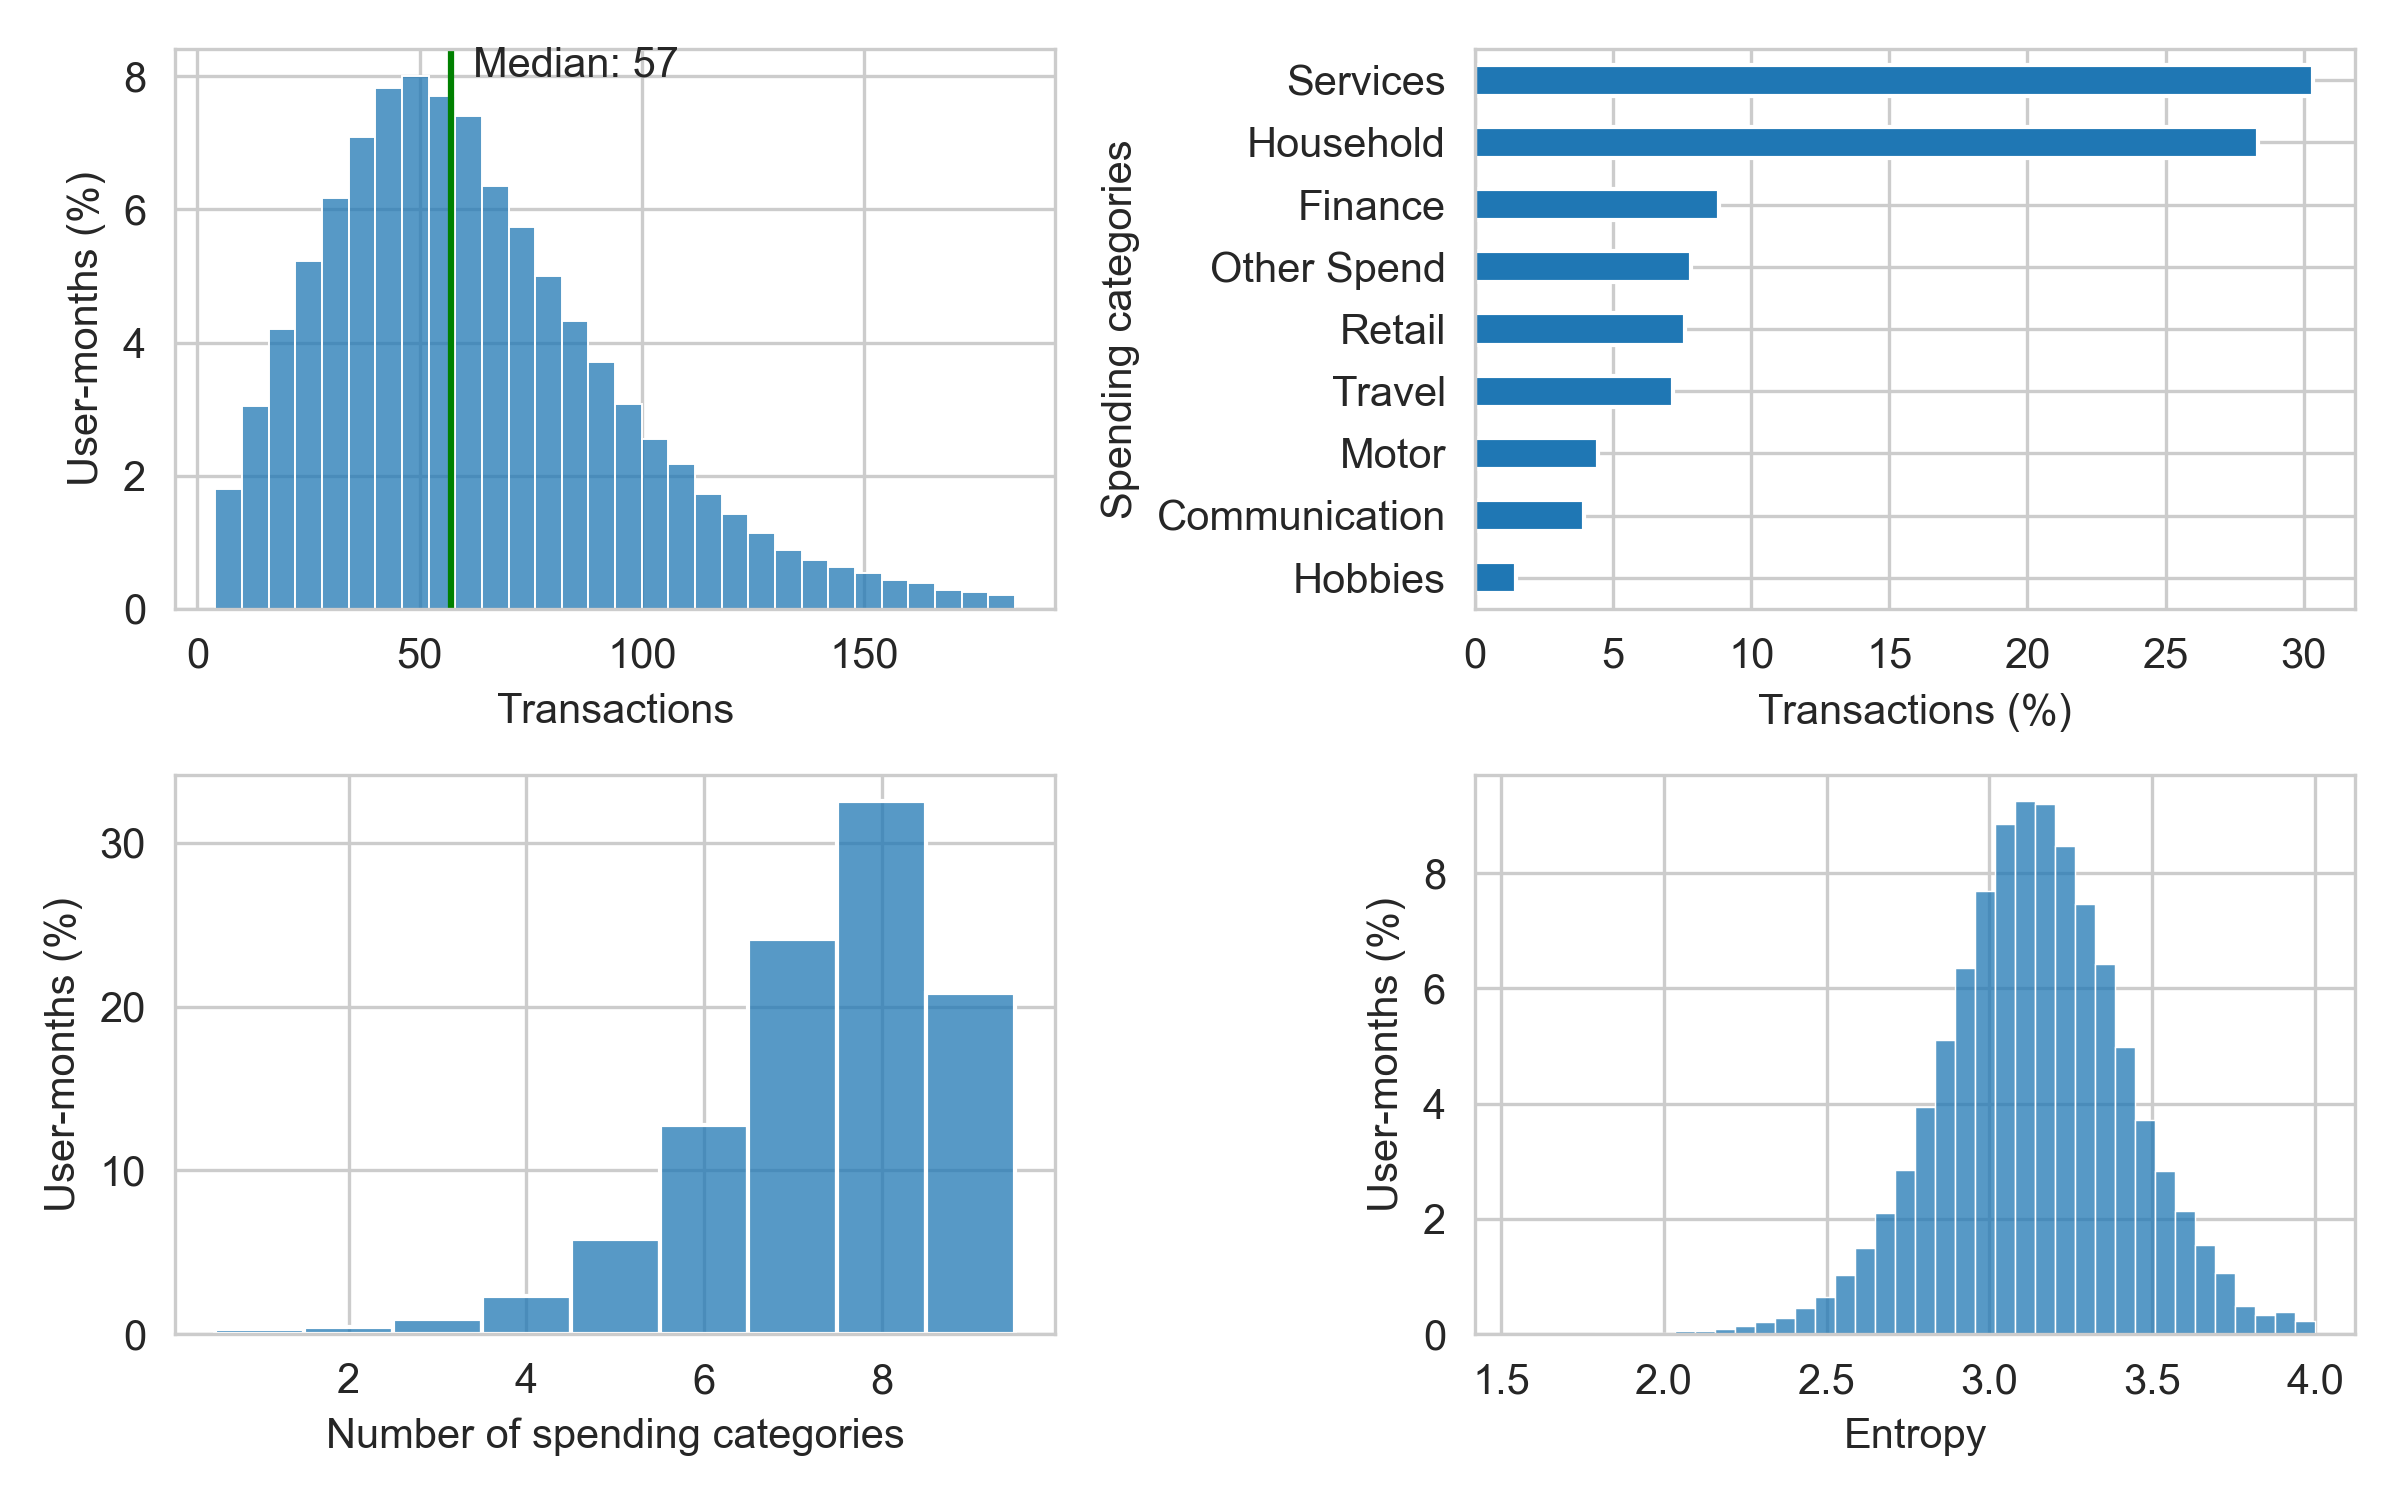
\includegraphics[width=\width]{\figdir/txns_breakdowns_and_entropy.png}
    \fignote{\width}{From top-left to bottom-right: distribution of spending
    transactions per user-month, breakdown of spending transactions into
spending categories; breakdown of number of spending categories spent on in
user-month; distribution of user-month entropy scores.}
\end{figure}

